\documentclass{article}
\usepackage[utf8]{inputenc}
\usepackage[russian]{babel}           
\usepackage[justification=centering]{caption}
\usepackage[backend=bibtex,sorting=none]{biblatex}
\usepackage{fontspec}
\usepackage[final]{graphicx}
\usepackage{tabularx,booktabs}
\newcolumntype{C}{>{\centering\arraybackslash}X} % centered version of "X" type
\setlength{\extrarowheight}{3pt}
\usepackage{float}
\usepackage{subcaption}
\usepackage{mathtools}
\usepackage{adjustbox}
\usepackage{listings}
\usepackage{array}
\usepackage{xcolor}
\usepackage{graphicx}
\usepackage{tikz}
\usepackage{pgfplots}
\usepackage{fontspec}
\usepackage{amssymb}
%\usepackage{unicode-math}
\graphicspath{{./images/}}


\definecolor{codegreen}{rgb}{0,0.6,0}
\definecolor{codegray}{rgb}{0.5,0.5,0.5}
\definecolor{codepurple}{rgb}{0.58,0,0.82}
\definecolor{backcolour}{rgb}{0.95,0.95,0.92}

\newcommand{\A}{\underline{A}}
\newcommand{\B}{\underline{B}}
\newcommand{\und}[1]{\underline{#1}}
\newcommand{\sqft}[3]{#1_{#2}, \ldots, #1_{#3}}

\usepackage[%
        a4paper,%
        includehead,%
        left=2cm,%
        top=0.95cm,%
        right=2cm,%
        bottom=1.65cm,%
        headheight=0.7cm,%
        headsep=0.3cm,%
        footskip=0.8cm]{geometry}
\special{papersize=210mm,297mm}

\lstdefinestyle{mystyle}{
    language=C++,
    backgroundcolor=\color{white},   
    commentstyle=\color{codegreen},
    keywordstyle=[1]{\color{magenta}},
    keywordstyle=[2]{\color{blue}},
    numberstyle=\color{codegray},
    stringstyle=\color{codepurple},
    basicstyle=\ttfamily\footnotesize,
    keywords=[1]{*,<,>,algo, params, param, block, vertex, arg, in},            % if you want to add more keywords to the set
    keywords=[2]{*, id, name, condition, dims, type, val, bsrc, src, value},            % if you want to add more keywords to the set
    breakatwhitespace=false,         
    breaklines=true,                 
    captionpos=b,                    
    keepspaces=true,                 
    numbers=left,                    
    numbersep=10pt,
    xleftmargin=7mm,
    xrightmargin=0mm,
    showspaces=false,                
    showstringspaces=false,
    showtabs=false,                  
    tabsize=4
}
\lstset{style=mystyle}

\lstset{linewidth=1.1\linewidth}
\setmainfont{Times New Roman}
\setmonofont{Monaco}
\title{Отчёт по практическому заданию (2) в рамках курса\\«Суперкомпьютерное моделирование и технологии»\\Вариант 5}
\author{Никифоров Никита Игоревич, гр. 621\\nickiforov.nik@gmail.com}
\date{Октябрь 2022}
\pgfplotsset{compat=1.17}
            
\renewcommand{\baselinestretch}{1.5}
\begin{document}
\maketitle
\newpage
\section{Задача}
    Необходимо реализовать численный метод Монте-Карло нахождения значения интеграла
    в заданной области. Для реализации метода предлагается использовать языки программирования 
    {\tt C/C++}, с использованием библиотеки параллельного вычисления {\tt MPI}.

    Необходимо провести исследование реализованного численного метода для
    заданного интеграла, области и точности 
    на параллельных вычислительных системах ВМК МГУ: {\tt IBM Blue Gene/P}, {\tt IBM Polus}
\section{Математическая постановка задачи}
    Пусть функция \(f(x, y, z) = x^3*y^2*z\)~--- непрерывна в ограниченной замкнутой области \(G \subset \mathbb{R}^3\).
    Требуется вычислить определённый интеграл:
    \begin{equation}
        I\ =\ \iiint_G f(x, y, z)\ dxdydz = \iiint_G x^3*y^2*z\ dxdydz,
        \label{eq:integ}
    \end{equation}
    где область \(G={(x,y,z):\ −1 \leq x \leq 0,\ −1\leq y \leq 0,\ −1\leq z \leq 0}\)
\section{Численный метод решения задачи (Монте-Карло)}
    Пусть заданная область \(G\) ограниченна параллелепипедом \(P:\ a_1 \leq x \leq b_2,\ a_2 \leq y \leq b_2,\ a_3 \leq z \leq b_3\)
    Рассмотрим функцию определённую на параллелепипеде \(P\):
    \begin{equation}
        F(x, y, z)\ =\
        \begin{cases}
            f(x, y, z), & (x, y, z) \in G\\
            0         , & (x, y, z) \notin G\\
        \end{cases}
        \label{eq:funcF}
    \end{equation}

    Преобразуем искомый интеграл~\ref{eq:integ} - подставив функцию~\ref{eq:funcF}.
    
    \begin{equation}
        I\ =\ \iiint_G f(x, y, z)\ dxdydz\ =\ \iiint_P F(x, y, z)\ dxdydz,
        \label{eq:integF}
    \end{equation}

    Пусть \(p_1:\ (x_1, y_1, z_1),\ p_2:\ (x_2, y_2, z_2),\ldots, p_n:\ (x_n, y_n, z_n)\)~---
    случайные точки равномерно распределённые по области \(P\). Тогда в качестве приближённого
    значения интеграла~\ref{eq:integF} предлагается использовать выражение:
    \begin{equation}
        I \approx |P| * \frac{1}{n} *\sum_{i=1}^n F(p_i),
    \end{equation}
    где \(|P|\) — объём параллелепипеда \(P\), \(|P| = (b_1 − a_1)(b_2 − a_2)(b_3 − a_3)\).
\section{Аналитическое решение задачи}
    Найдём аналитически интеграл~\ref{eq:integ}:
    \begin{equation}
        \begin{aligned}
        I &= \iiint_G x^3*y^2*z\ dxdydz\ = \int_{-1}^{0} dx\int_{-1}^{0} dy \int_{-1}^{0} x^3*y^2*z\ dz\ =\\
          &\frac{x^4}{4}\biggr\rvert_{-1}^{0}\frac{y^3}{3}\biggr\rvert_{-1}^{0}\frac{z^2}{2}\biggr\rvert_{-1}^{0}\ =\ 
            \frac{1}{24} * x^4y^3z^2\biggr\rvert_{-1}^{0}\ =\ \frac{1}{24} \approx 0.0416(6)
        \end{aligned}
    \end{equation}
\section{Программная реализация}
    Для программной реализации предложенного метода используется язык {\tt C++}, а также 
    библиотека параллельного программирования {\tt MPI}.
    Программа разделяется на независимые процессы, каждый из которых генерирует свой набор 
    из 100 случайных точек, и считает свою частичную сумму.
    Принципиально алгоритм состоит из следующих шагов:
    \begin{enumerate}
        \item Каждый процесс генерируют набор из 100 случайных точек.
        \item Каждый процесс считает сумму \(S_j = \sum_{i=1}^{n} F(p_i)\), 
            где \(j\) - ранк процесса, \(n = 100\) - количество случайных точек, 
            генерируемых процессом за итерацию.
        \item C использованием функции {\tt MPI\_AllReduce}, 
            происходит вычисление суммы по всем процессам: 
            \(S_{global} = \sum_{j = 0}^{size - 1} S_j.\),
            где \(size\) - количество независимых {\tt MPI} процессов.
        \item В каждом процессе вычисляется приближённое значение интеграла:
            \(I_{global} = |P| * \frac{1}{n} * S_{global}\).
        \item Вычисляется ошибка: \(err = |I_{global} - I_{analitical}|\).
        \item Если ошибка меньше заданной вычисление прекращается, если больше,
            то алгоритм повторяется.
    \end{enumerate}
\begin{lstlisting}
std::pair<double, int64_t>  monte_carlo(std::mt19937 &gen, 
                                        std::uniform_real_distribution<> &dis, 
                                        double eps, double solution, double volume, 
                                        double (*func)(Point)) {
    double integ = 0.0;
    double err = std::abs(integ - solution);
    double global_sum = 0.0;
    int64_t point_counter = 0;

    while (err > eps) {
        double local_sum = 0;//global_sum;
        
        for (int i = 0; i < POINTS_PER_CPU; i++) {
            local_sum += func(Point(dis, gen));
        }
        
        double now_sum = 0.0;
        MPI_Allreduce(&local_sum, &now_sum, 1, MPI_DOUBLE, MPI_SUM, MPI_COMM_WORLD);
        global_sum += now_sum;
        
        point_counter += POINTS_PER_CPU * size;
        integ = volume * global_sum / (point_counter + 0.0);
        err = std::abs(integ - solution);
    
    }

    return {integ, point_counter}; 
}
\end{lstlisting}
\section{Исследование программной реализации}
    Для исследования использовалась система Polus и домашний компьютер.
    Характеристики узла системы параллельного вычисления Polus (на данный момент имеет в работе 3 узла):
    \begin{itemize}
        \item 2 десятиядерных процессора IBM POWER8 (каждое ядро имеет 8 потоков) всего 160 потоков
        \item Общая оперативная память 256 Гбайт (в узле 5 оперативная память 1024 Гбайт) с ЕСС контролем
        \item 2 х 1 ТБ 2.5” 7K RPM SATA HDD
        \item 2 x NVIDIA Tesla P100 GPU, 16Gb, NVLink
        \item 1 порт 100 ГБ/сек
    \end{itemize}

    Характеристики домашнего PC:
    \begin{itemize}
        \item 1 шестнадцати ядерный процессор AMD Ryzen 5950X, всего 32 потока на частоте 4.4Ghz
        \item Оперативная память 32 Гбайт
        \item SSD NVMe Samsung 500 ГБ
        \item AMD RX 5600XT
    \end{itemize}

    Для каждого значения требуемой точности \(eps = \{1.5e-6, 5.0e-6, 3.0e-5\}\) 
    и каждого количества процессов \(cpus = \{1, 4, 8, 16, 32\}\) проводилось по 10 запусков,
    значения усреднялись.

    Ускорение считалось как отношение времени вычисления одной точки при разном 
    количестве MPI процессов, что позволяет исключить случайность процесса при вычислении ускорения.
    А также как отношение общего времени выполнения на одном MPI-процессе ко времени вычисления на заданном количестве MPI-процессов.
    Составим таблицу для системы Polus:
    \begin{table*}[!t]
        \centering
        \caption{Результаты исследования на машине Polus}\label{tab:tab1}
        \begin{tabularx}{\textwidth}{@{}l*{10}{C}c@{}} %{|m{3.5cm}|m{2.5cm}|m{2cm}|m{3.5cm}|m{4cm}|}
            \toprule
            \bf Точность & \bf число MPI процессов  & \bf Время работы (с) & \bf Ускорение по времени & \bf Ускорение & \bf Ошибка \\
                \midrule
                \(3.0 * 10^{-5}\) & 1  & 0.024625 & 1    & 1     & 0.000012\\
                \(3.0 * 10^{-5}\) & 4  & 0.021700 & 1.13 & 3.09  & 0.000013\\
                \(3.0 * 10^{-5}\) & 8  & 0.053036 & 0.46 & 4.83  & 0.000018\\
                \(3.0 * 10^{-5}\) & 16 & 0.081705 & 0.30 & 7.56  & 0.000019\\
                \(3.0 * 10^{-5}\) & 32 & 0.093178 & 0.26 &12.27 & 0.000017\\
                \midrule
                \(5.0 * 10^{-6}\) & 1  & 0.745260 & 1     & 1     & 0.000003 \\
                \(5.0 * 10^{-6}\) & 4  & 0.068947 & 10.8  & 3.09  & 0.000002 \\
                \(5.0 * 10^{-6}\) & 8  & 0.345431 & 2.15  & 4.76  & 0.000003 \\
                \(5.0 * 10^{-6}\) & 16 & 0.043465 & 17.14 & 9.84  & 0.000003 \\
                \(5.0 * 10^{-6}\) & 32 & 0.072755 & 10.24 & 14.28 & 0.000003 \\
                \midrule
                \(1.5 * 10^{-6}\) & 1  & 27.415805 & 1      & 1     & 8.013453e-07 \\
                \(1.5 * 10^{-6}\) & 4  &  2.434363 & 11.26  & 3.13  & 9.394432e-07 \\
                \(1.5 * 10^{-6}\) & 8  &  0.223442 & 122.69 & 5.46  & 8.698047e-07 \\
                \(1.5 * 10^{-6}\) & 16 &  4.428387 & 6.19   & 10.35 & 7.874600e-07 \\
                \(1.5 * 10^{-6}\) & 32 &  0.192503 & 142.41 & 15.12 & 6.611632e-07 \\
                \bottomrule
            \end{tabularx}
        \end{table*}
        \clearpage
\begin{figure*}[!t]
\centering
\begin{subfigure}[b]{0.49\textwidth}
    \centering
    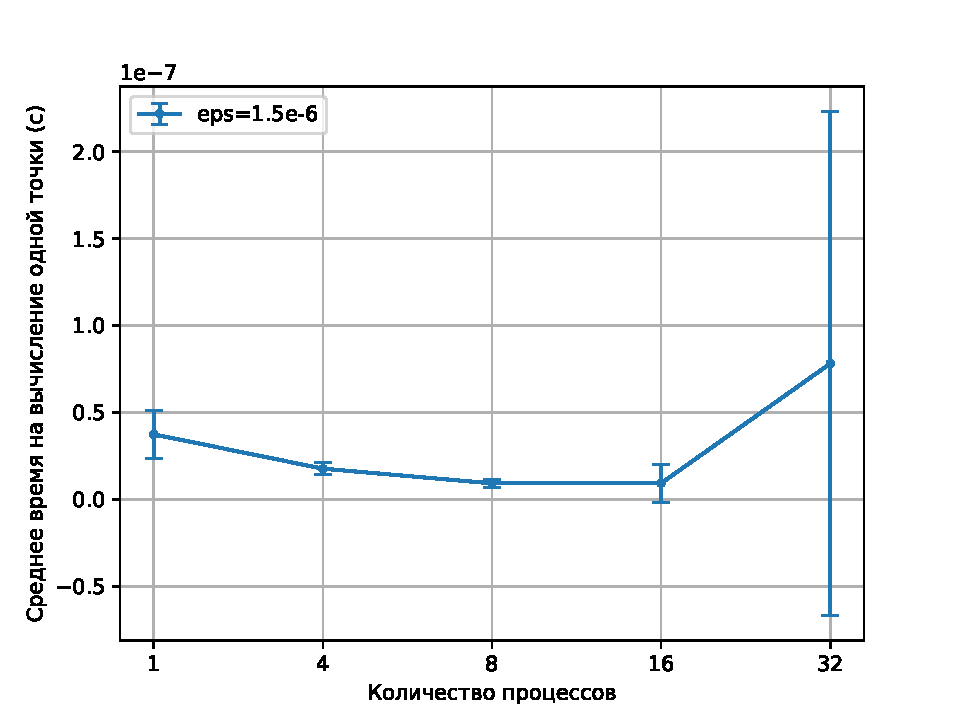
\includegraphics[width=\textwidth,trim=0 0 0 0,clip]{1.5e-6_home_pc_time_pp.pdf}
    \caption{На домашнем компьютере}
    \label{img:1.1}
\end{subfigure}
\begin{subfigure}[b]{0.49\textwidth}
    \centering
    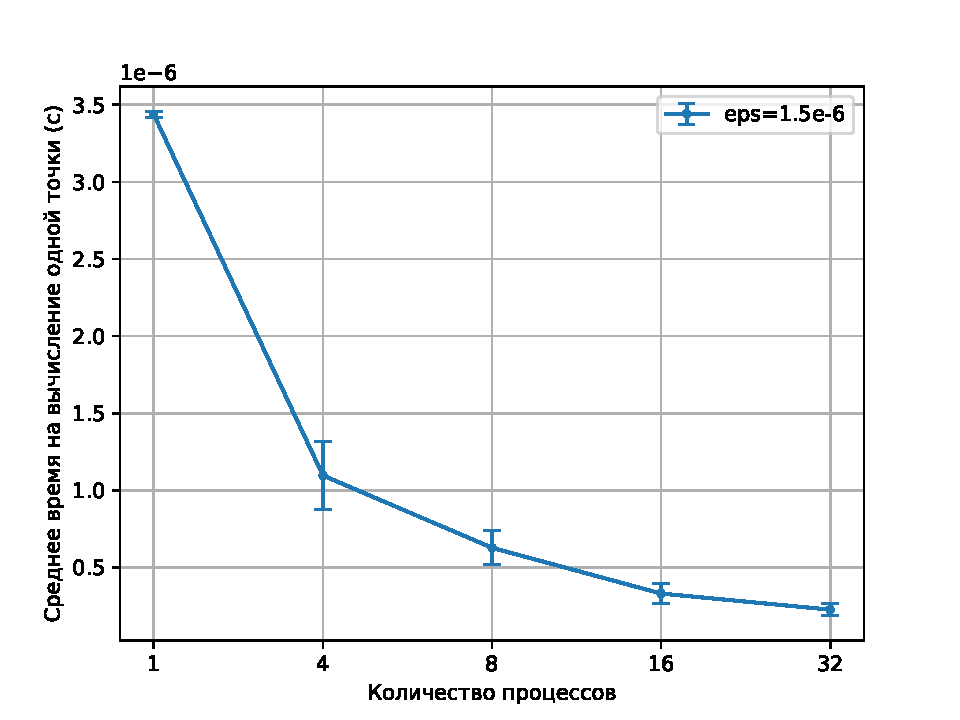
\includegraphics[width=\textwidth,trim=0 0 0 0,clip]{1.5e-6_polus_time_pp.pdf}
    \caption{На системе Polus}
    \label{img:1.2}
\end{subfigure}
\caption{График зависимость времени вычисления одной точки от количества процессов MPI}
\end{figure*}

\begin{figure*}[!t]
\centering
\begin{subfigure}[b]{0.49\textwidth}
    \centering
    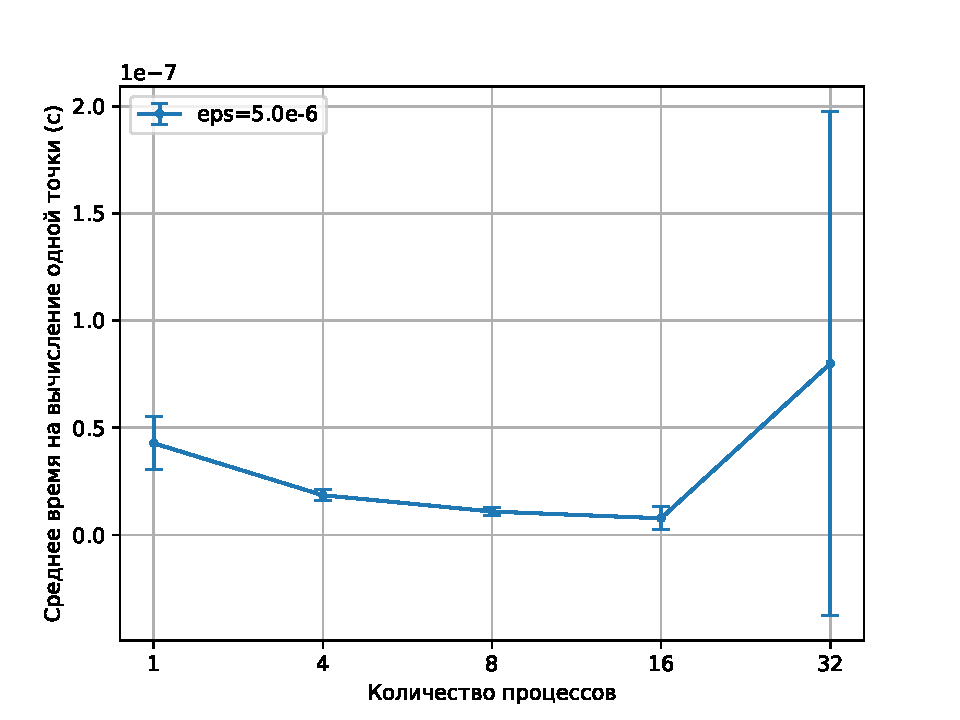
\includegraphics[width=\textwidth,trim=0 0 0 0,clip]{5.0e-6_home_pc_time_pp.pdf}
    \caption{На домашнем компьютере}
    \label{img:2.1}
\end{subfigure}
\begin{subfigure}[b]{0.49\textwidth}
    \centering
    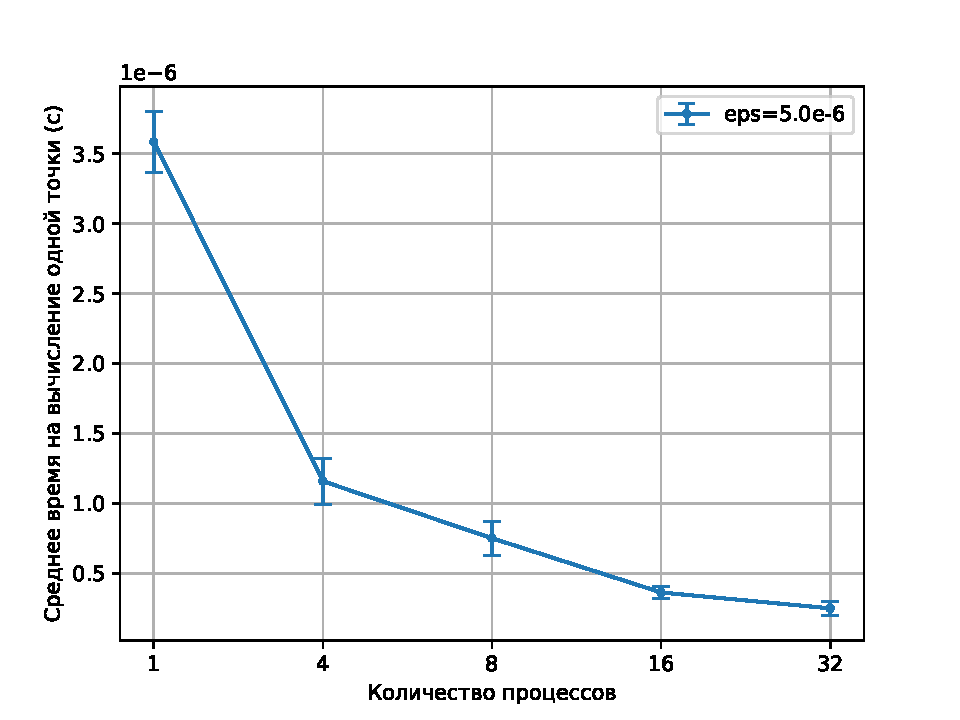
\includegraphics[width=\textwidth,trim=0 0 0 0,clip]{5.0e-6_polus_time_pp.pdf}
    \caption{На системе Polus}
    \label{img:2.2}
\end{subfigure}
\caption{График зависимость времени вычисления одной точки от количества процессов MPI}
\end{figure*}

\begin{figure*}[!t]
\centering
\begin{subfigure}[b]{0.49\textwidth}
    \centering
    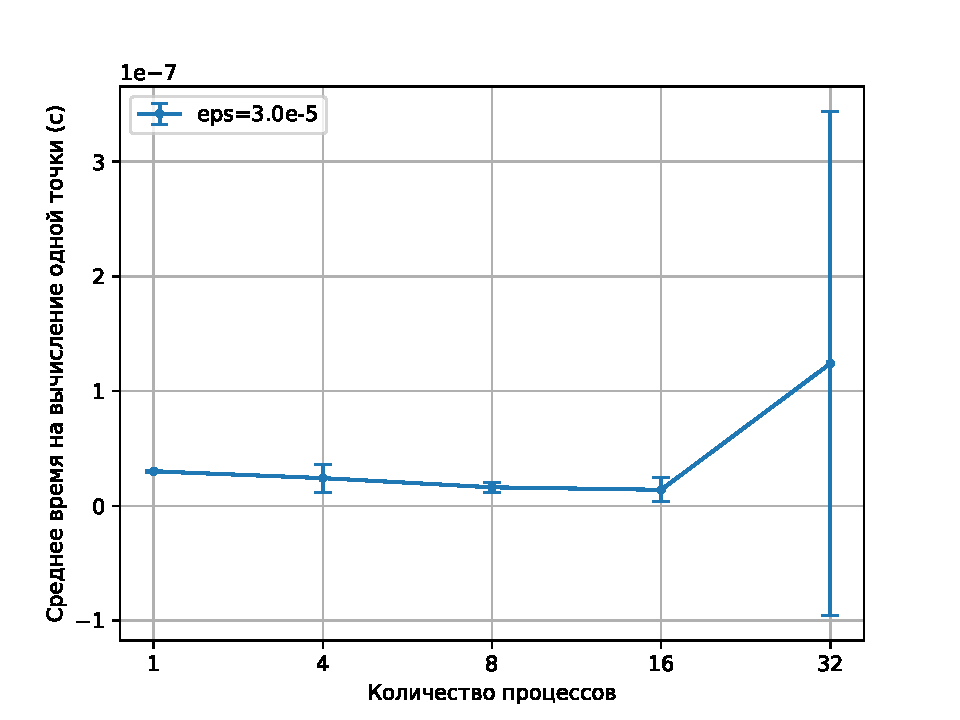
\includegraphics[width=\textwidth,trim=0 0 0 0,clip]{3.0e-5_home_pc_time_pp.pdf}
    \caption{На домашнем компьютере}
    \label{img:3.1}
\end{subfigure}
\begin{subfigure}[b]{0.49\textwidth}
    \centering
    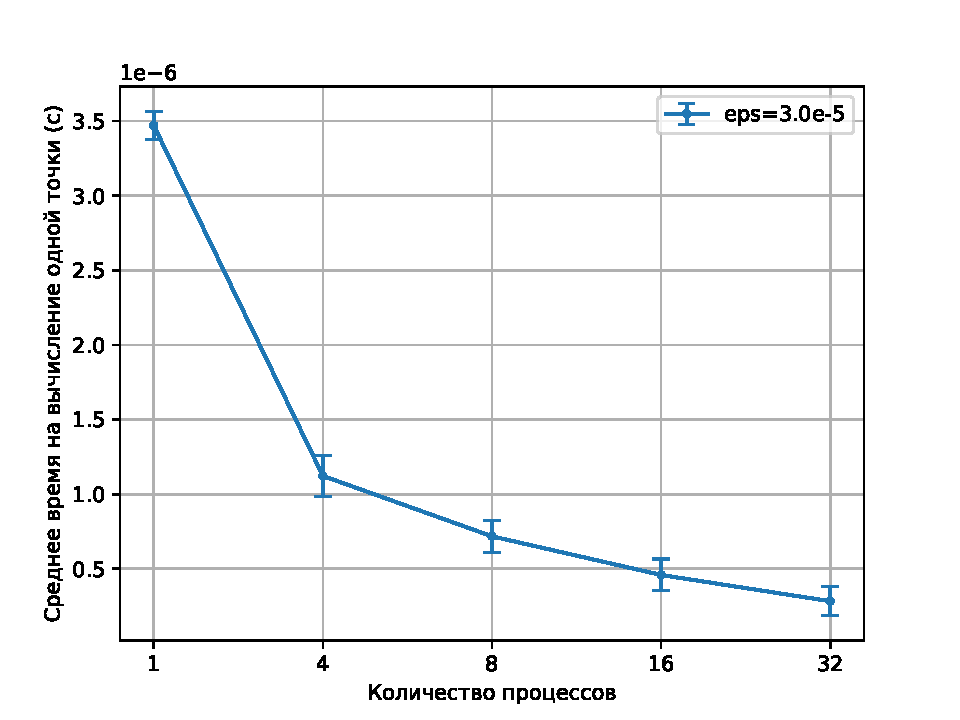
\includegraphics[width=\textwidth,trim=0 0 0 0,clip]{3.0e-5_polus_time_pp.pdf}
    \caption{На системе Polus}
    \label{img:3.2}
\end{subfigure}
\caption{График зависимость времени вычисления одной точки от количества процессов MPI}
\end{figure*}

\begin{figure*}[!t]
\centering
\begin{subfigure}[b]{0.49\textwidth}
    \centering
    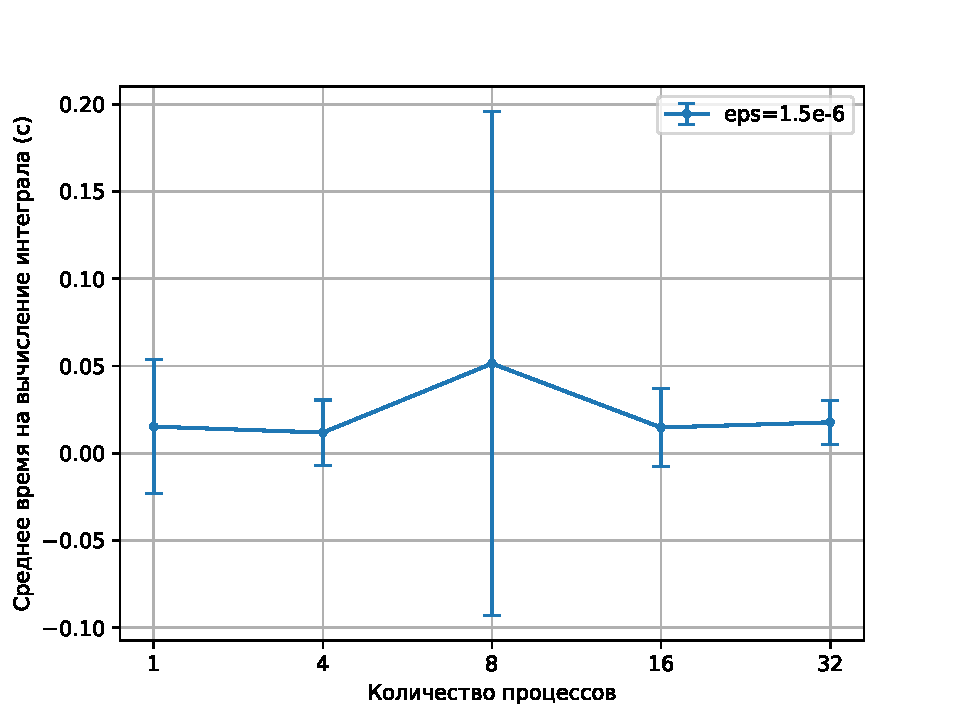
\includegraphics[width=\textwidth,trim=0 0 0 0,clip]{1.5e-6_home_pc_time.pdf}
    \caption{На домашнем компьютере}
    \label{img:1.1}
\end{subfigure}
\begin{subfigure}[b]{0.49\textwidth}
    \centering
    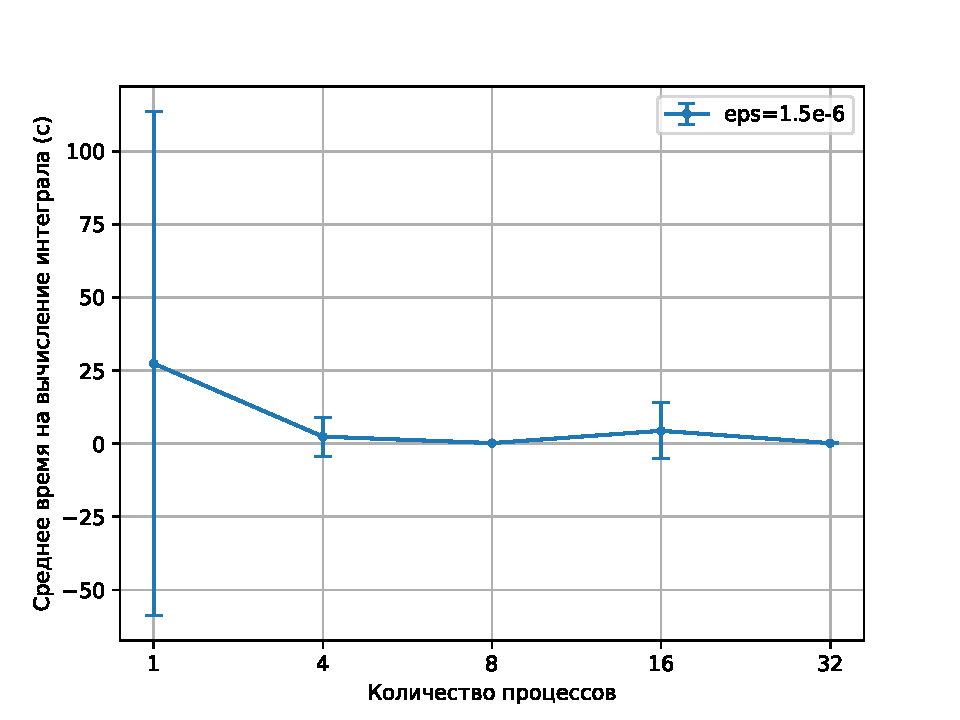
\includegraphics[width=\textwidth,trim=0 0 0 0,clip]{1.5e-6_polus_time.pdf}
    \caption{На системе Polus}
    \label{img:1.2}
\end{subfigure}
\caption{График зависимость времени вычисления значения интеграла от количества процессов MPI}
\end{figure*}

\begin{figure*}[!t]
\centering
\begin{subfigure}[b]{0.49\textwidth}
    \centering
    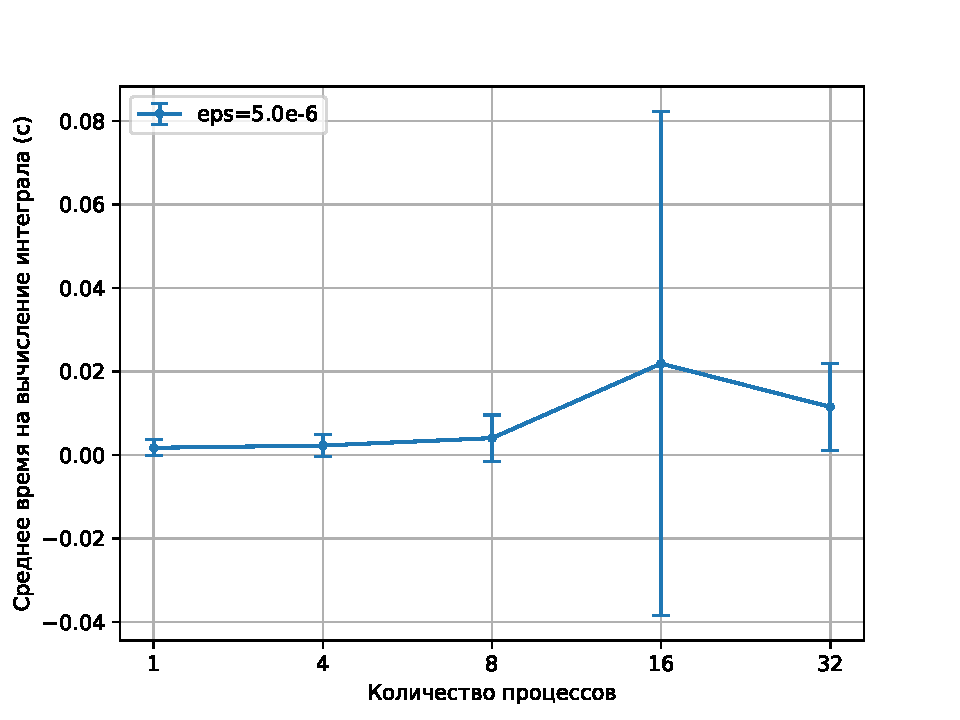
\includegraphics[width=\textwidth,trim=0 0 0 0,clip]{5.0e-6_home_pc_time.pdf}
    \caption{На домашнем компьютере}
    \label{img:2.1}
\end{subfigure}
\begin{subfigure}[b]{0.49\textwidth}
    \centering
    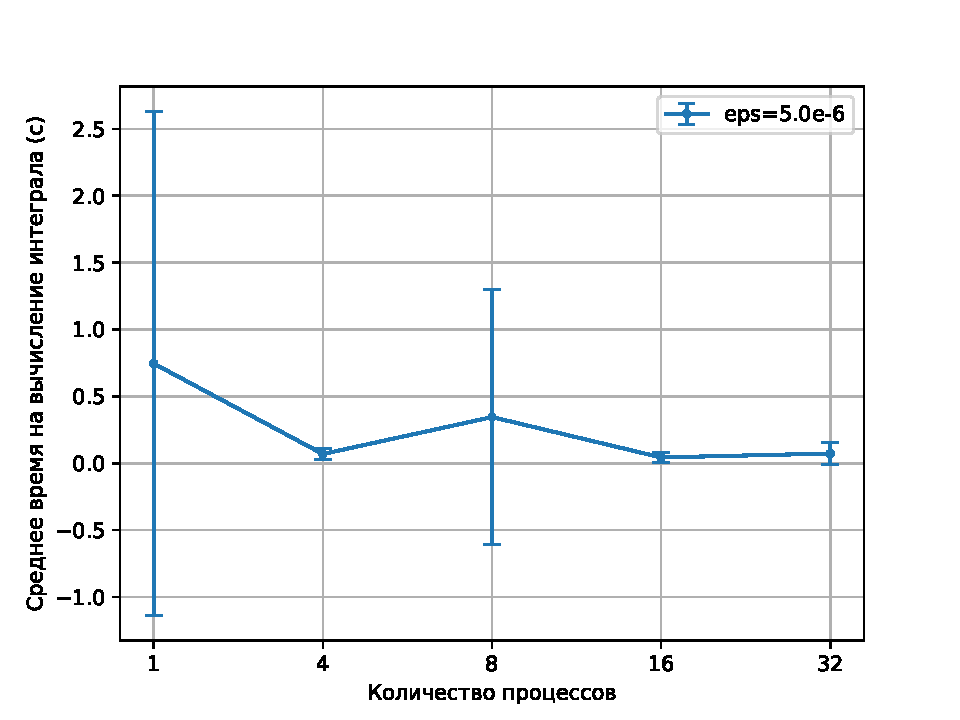
\includegraphics[width=\textwidth,trim=0 0 0 0,clip]{5.0e-6_polus_time.pdf}
    \caption{На системе Polus}
    \label{img:2.2}
\end{subfigure}
\caption{График зависимость времени вычисления значения интеграла  от количества процессов MPI}
\end{figure*}

\begin{figure*}[!t]
\centering
\begin{subfigure}[b]{0.49\textwidth}
    \centering
    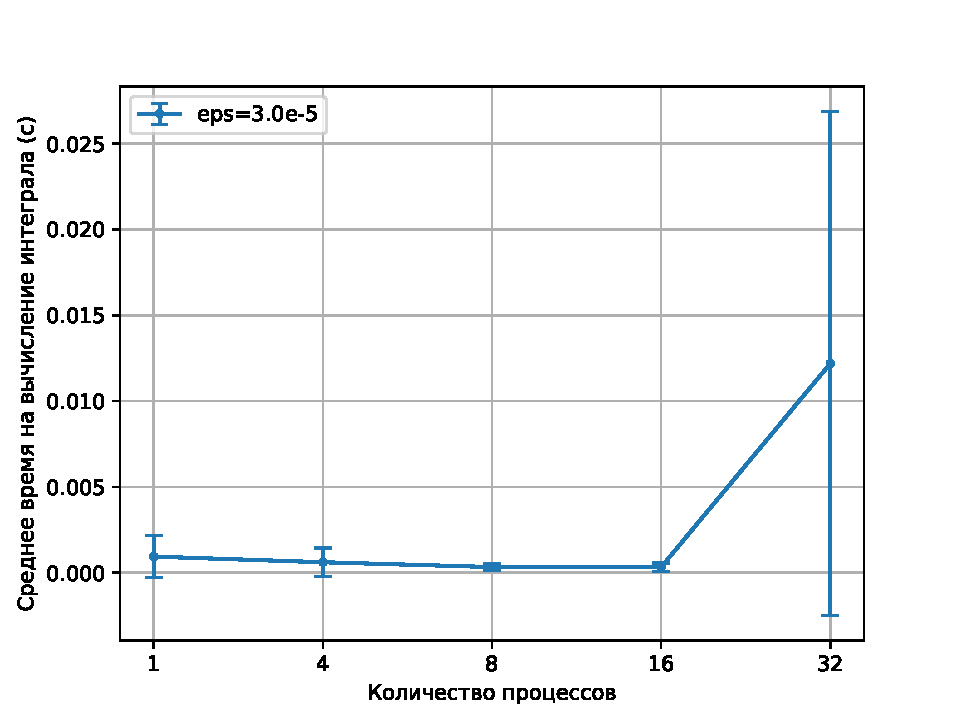
\includegraphics[width=\textwidth,trim=0 0 0 0,clip]{3.0e-5_home_pc_time.pdf}
    \caption{На домашнем компьютере}
    \label{img:3.1}
\end{subfigure}
\begin{subfigure}[b]{0.49\textwidth}
    \centering
    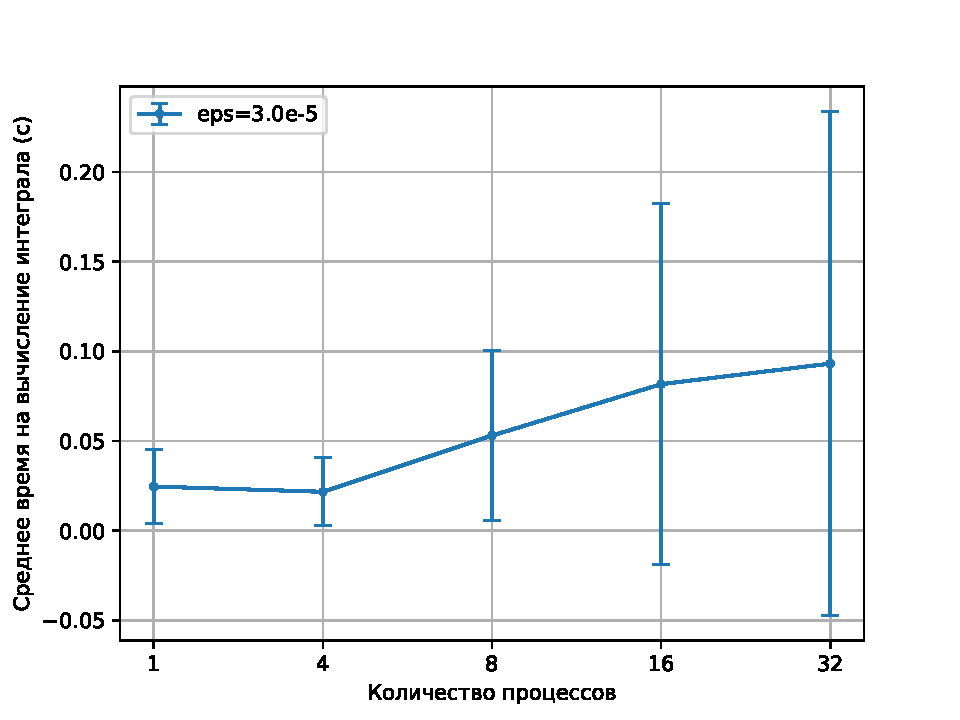
\includegraphics[width=\textwidth,trim=0 0 0 0,clip]{3.0e-5_polus_time.pdf}
    \caption{На системе Polus}
    \label{img:3.2}
\end{subfigure}
\caption{График зависимость времени вычисления значения интеграла от количества процессов MPI}
\end{figure*}
\end{document}
